\chapter{Release 2 : Supervision r\'eseau, Cartographie interactive et Temps r\'eel}
\label{chap:sprint_superv}

\section*{Introduction}
Ce quatri\`eme chapitre retrace la r\'ealisation de la deuxi\`eme release du projet, correspondant aux it\'erations \textbf{S4 \`a S7}. Cette \'etape constitue le c\oe ur m\'etier op\'erationnel de la plateforme : elle permet aux \'equipes de supervision et aux techniciens de visualiser l'\'etat physique et logique du r\'eseau fibre optique sur une carte g\'eographique interactive multi-couches, de recevoir instantan\'ement les \'ev\'enements et alertes de coupure via WebSockets, et de piloter les indicateurs de performance \`a travers un tableau de bord d\'edi\'e.

\section{Backlog de la Release 2}
Le tableau~\ref{tab:backlog-release2} r\'esume les objectifs planifi\'es pour les sprints S4 \`a S7.

\begin{table}[H]
\centering
\begin{tabular}{|p{8.5cm}|c|c|}
\hline
\textbf{\'El\'ement du Backlog} & \textbf{Priorit\'e} & \textbf{Sprint} \\
\hline
Mod\'elisation g\'eospatiale des zones, NRO, FDT, contrats et liaisons optiques & Haute & S4 \\
\hline
Indexation g\'eographique MongoDB (\textit{2dsphere}) et requ\^etes spatiales & Haute & S4 \\
\hline
Mise en place de la passerelle temps r\'eel Socket.IO et multiplexage par zones & Haute & S5 \\
\hline
D\'eveloppement du module cartographique mobile multi-couches avec \textit{flutter\_map} & Haute & S6 \\
\hline
Impl\'ementation des fiches d\'etaill\'ees et popups interactifs des entit\'es & Moyenne & S6 \\
\hline
Conception et r\'ealisation du tableau de bord KPI (\textit{fl\_chart}) et du centre d'alertes & Haute & S7 \\
\hline
\end{tabular}
\caption{Backlog d\'etaill\'e de la Release 2 (Sprints S4 \`a S7)}
\label{tab:backlog-release2}
\end{table}

\section{Raffinement des exigences et mod\'elisation UML}

\subsection{Diagramme de cas d'utilisation global de la Supervision R\'eseau}
La figure~\ref{fig:ch4-supervision-global} mod\'elise l'ensemble des cas d'utilisation associ\'es \`a la supervision, \`a la cartographie et \`a la r\'eception d'alertes.

\begin{figure}[H]
 \centering
 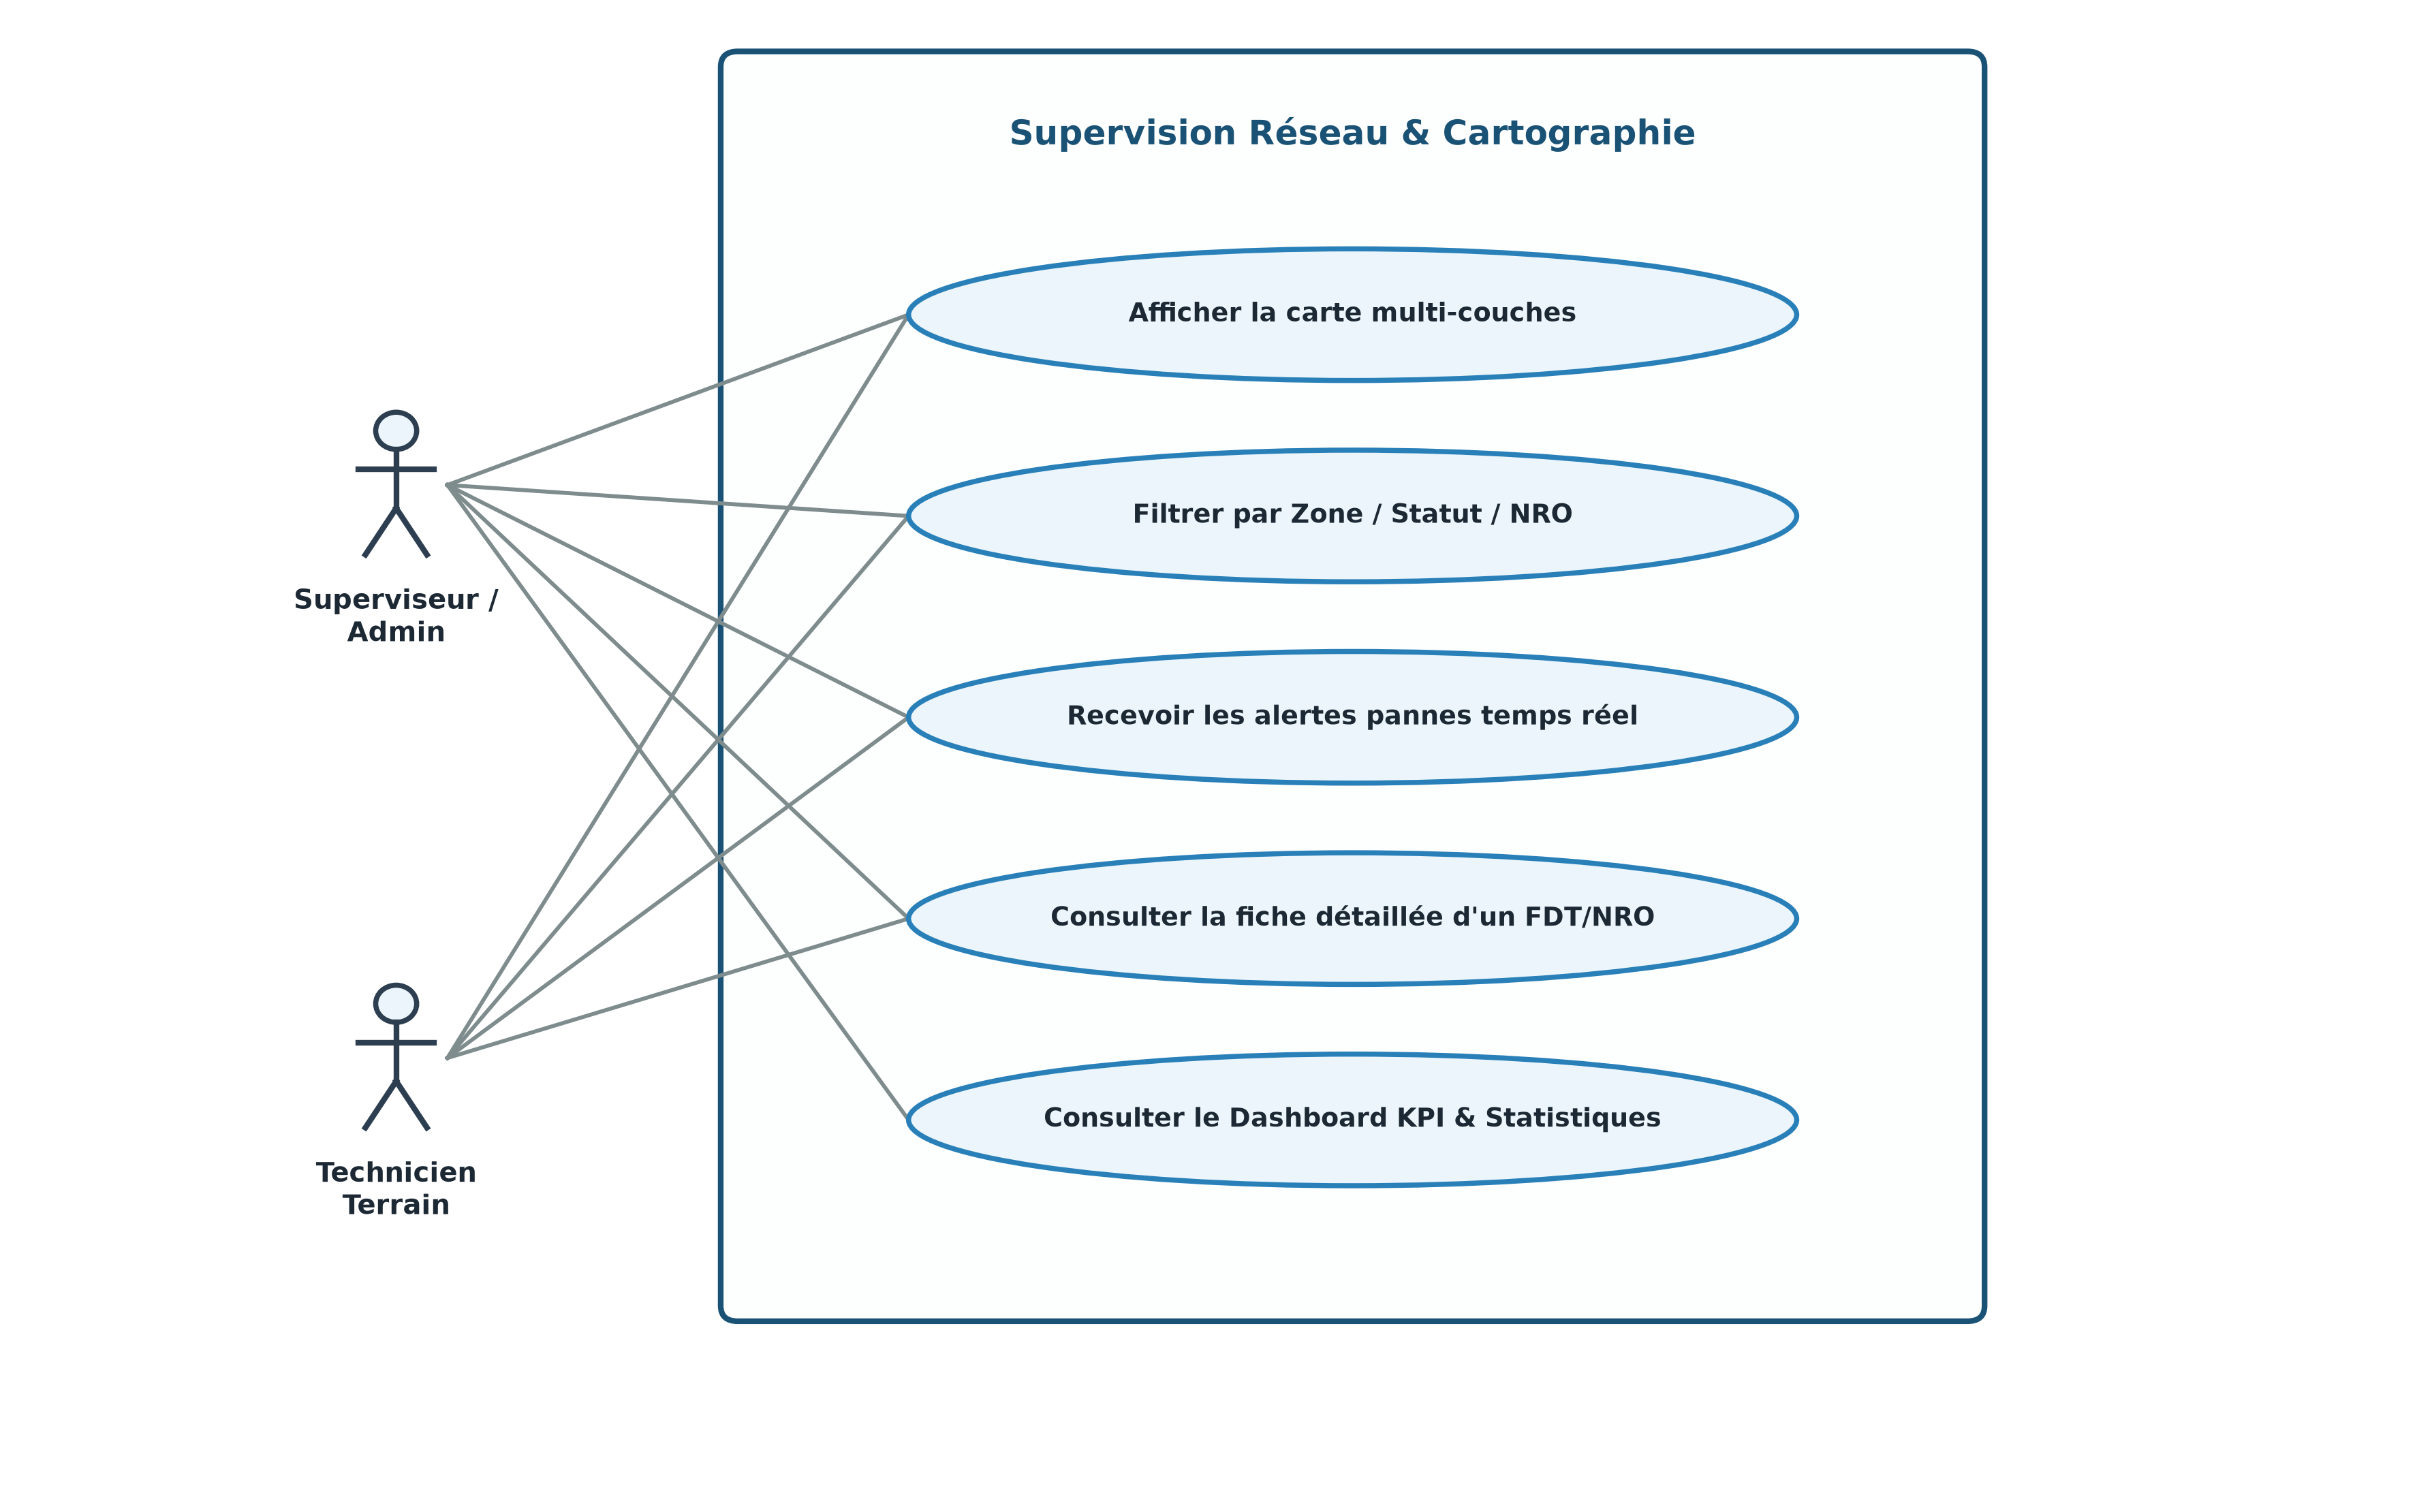
\includegraphics[width=14cm]{Images/ch4/network_supervision_usecase.png}
 \caption{Diagramme de cas d'utilisation global -- Supervision r\'eseau et Temps r\'eel}
 \label{fig:ch4-supervision-global}
\end{figure}

\subsection{Description textuelle du cas d'utilisation « Superviser le r\'eseau sur carte interactive »}
Le tableau~\ref{tab:ch4-map-refinement} d\'efinit le sc\'enario de supervision cartographique en conditions r\'eelles.

\begin{table}[H]
\centering
\begin{tabular}{|p{3.5cm}|p{10.5cm}|}
\hline
\textbf{Cas d'utilisation} & Superviser le r\'eseau sur carte interactive \\
\hline
\textbf{Acteurs} & Responsable de zone, Technicien, Administrateur \\
\hline
\textbf{Pr\'econditions} & L'utilisateur est authentifi\'e et autoris\'e sur le p\'erim\`etre g\'eographique consult\'e. \\
\hline
\textbf{Postconditions} & La carte g\'eographique affiche les couches activ\'ees (polygones de zones, NRO, FDT, clients, liaisons) avec leur statut op\'erationnel actualis\'e en direct. \\
\hline
\textbf{Sc\'enario nominal} & 
1. L'utilisateur ouvre l'\'ecran cartographique. \newline
2. L'application charge les donn\'ees g\'eospatiales via l'API REST filtr\'ees par la vue courante (\textit{Bounding Box}). \newline
3. L'utilisateur filtre les couches d'affichage (ex : masquer les FDT sains, n'afficher que les alertes critiques). \newline
4. L'utilisateur clique sur un \'equipement pour consulter sa fiche d\'etaill\'ee (capacit\'e, nombre d'abonn\'es, taux d'att\'enuation optique). \newline
5. En cas de survenance d'une panne, un \'ev\'enement WebSocket est re\c{c}u et met \`a jour la couleur du marqueur instantan\'ement sans rechargement de page. \\
\hline
\end{tabular}
\caption{Description textuelle du cas d'utilisation « Superviser le r\'eseau »}
\label{tab:ch4-map-refinement}
\end{table}

\subsection{Diagramme de s\'equence du flux temps r\'eel}
La figure~\ref{fig:ch4-realtime-seq} illustre la propagation d'un \'ev\'enement r\'eseau depuis son ingestion jusqu'\`a sa restitution dynamique sur le terminal mobile.

\begin{figure}[H]
 \centering
 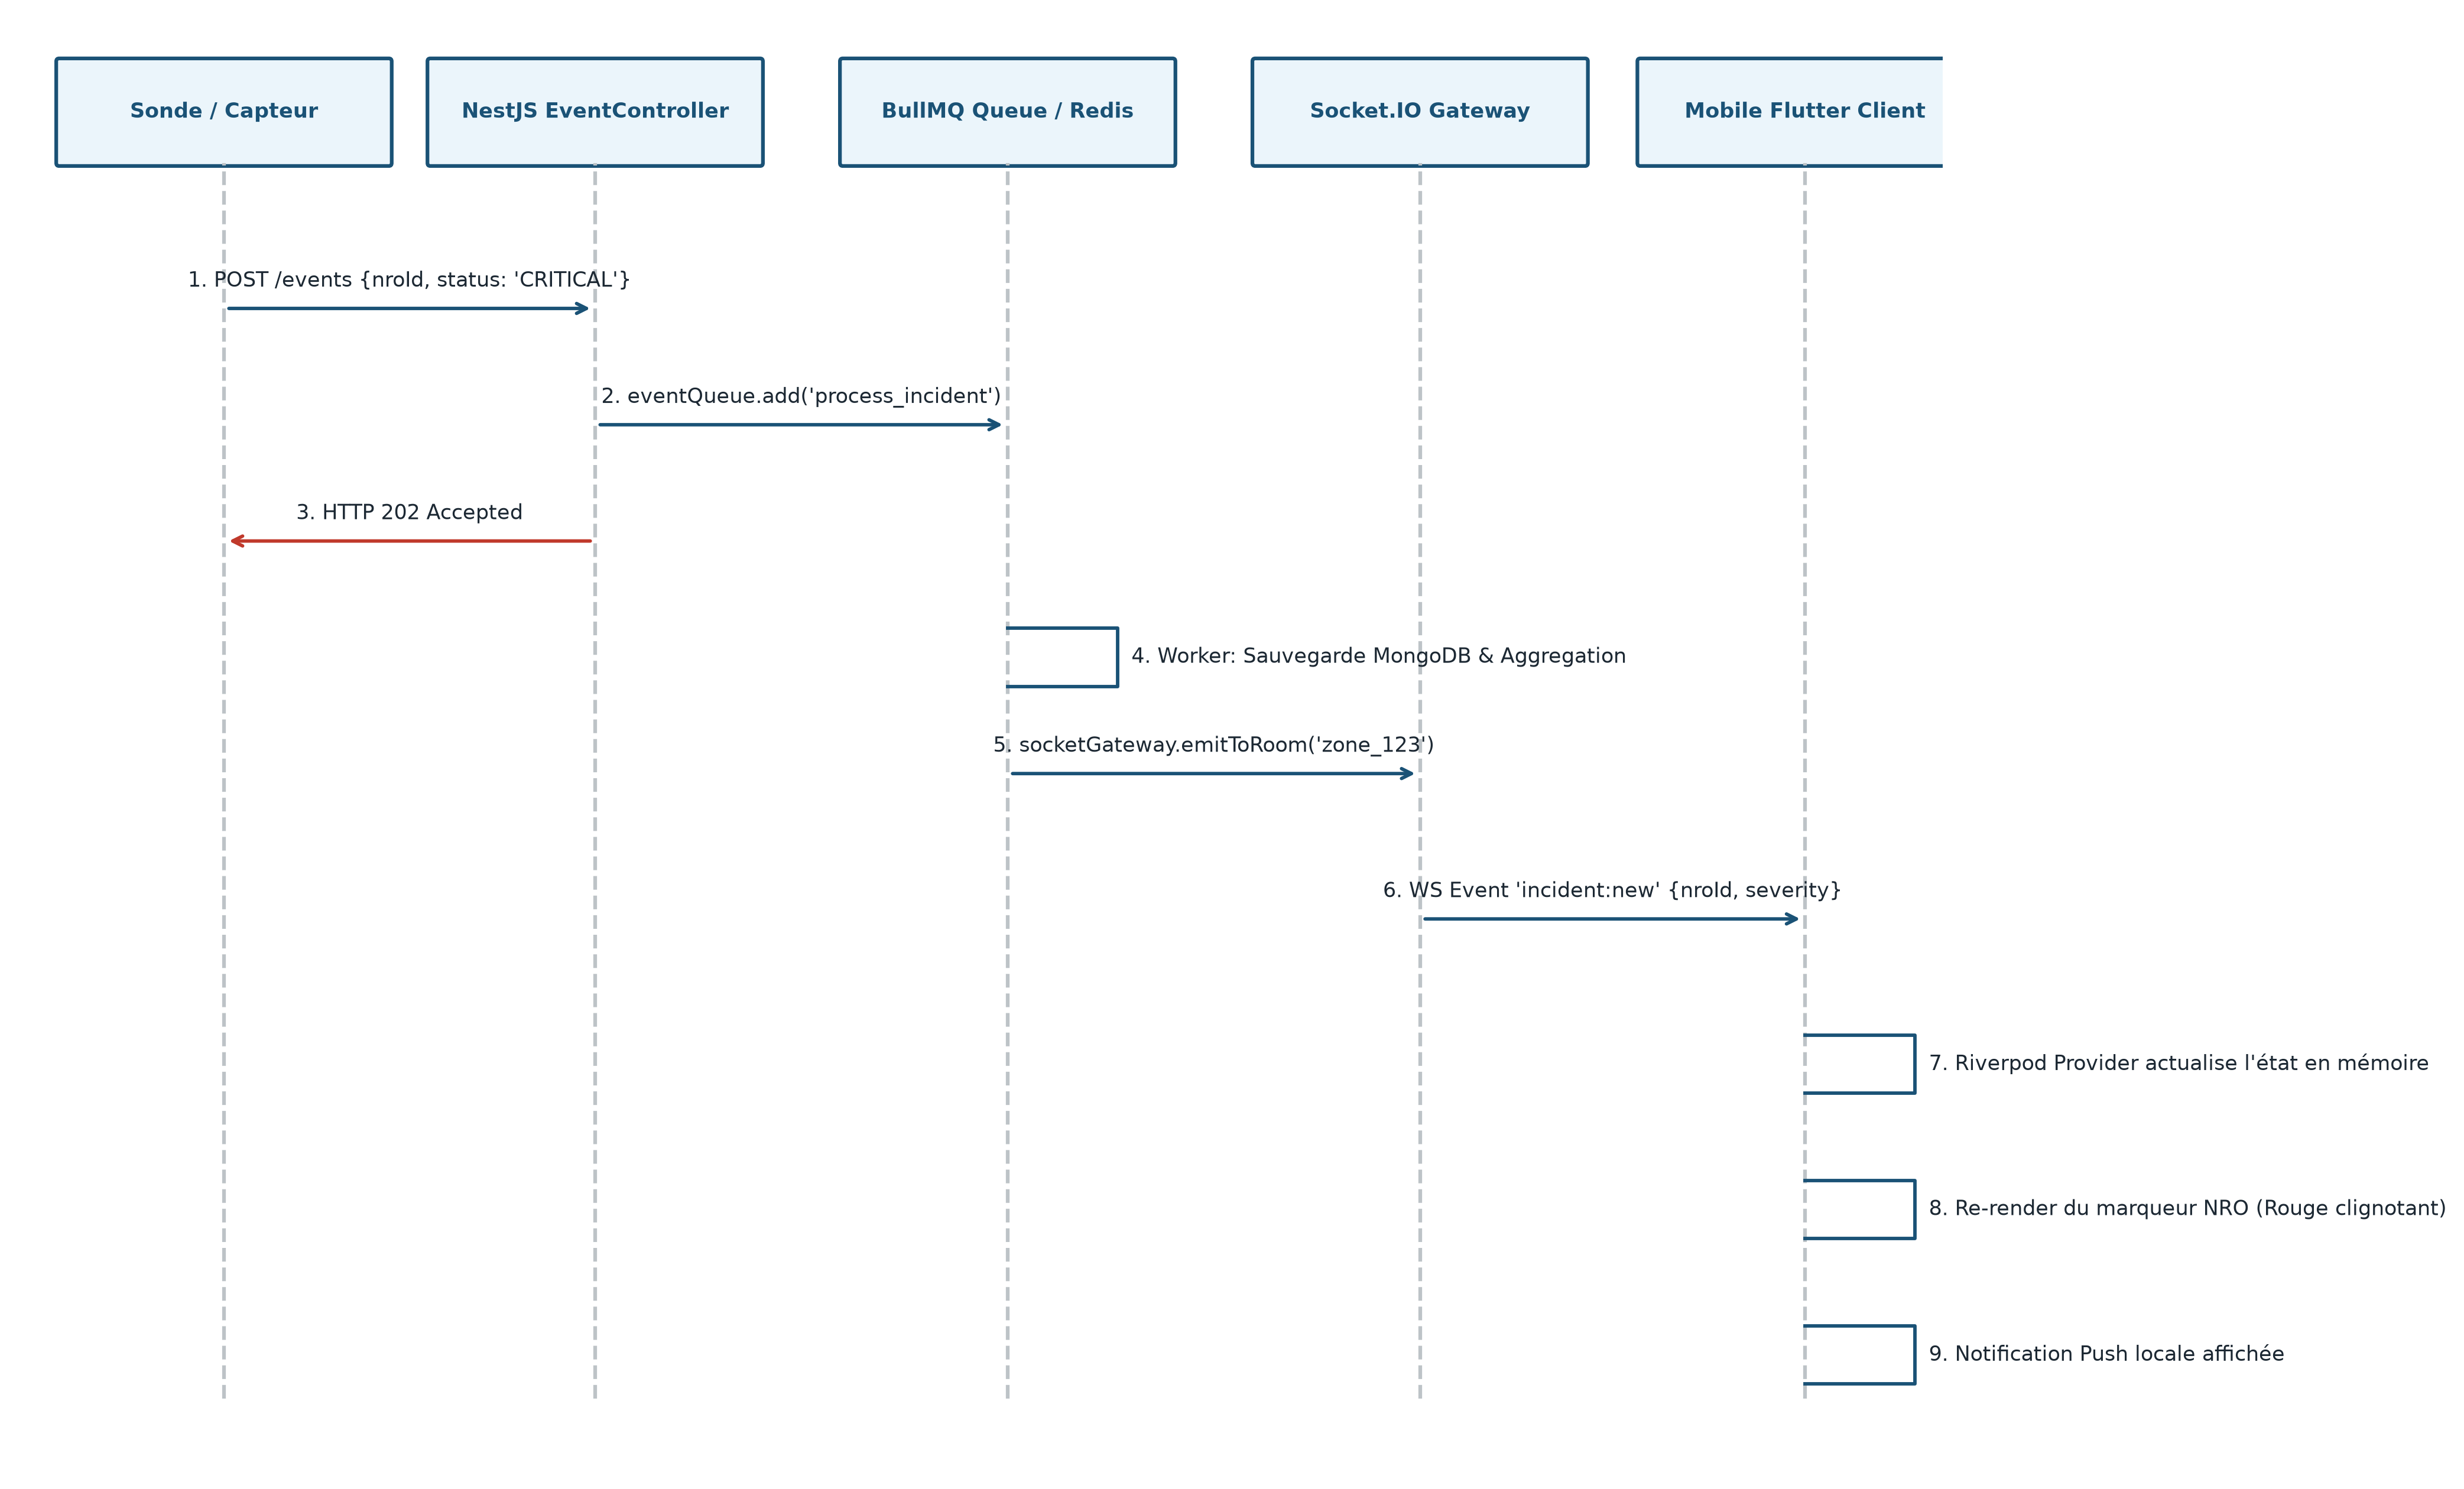
\includegraphics[width=15cm]{Images/ch4/realtime_sequence.png}
 \caption{Diagramme de s\'equence -- Traitement et diffusion temps r\'eel d'un \'ev\'enement}
 \label{fig:ch4-realtime-seq}
\end{figure}

\subsection{Diagramme de classes du domaine R\'eseau \& Cartographie}
La structure des entit\'es r\'eseau est illustr\'ee dans la figure~\ref{fig:ch4-map-layers-class}.

\begin{figure}[H]
 \centering
 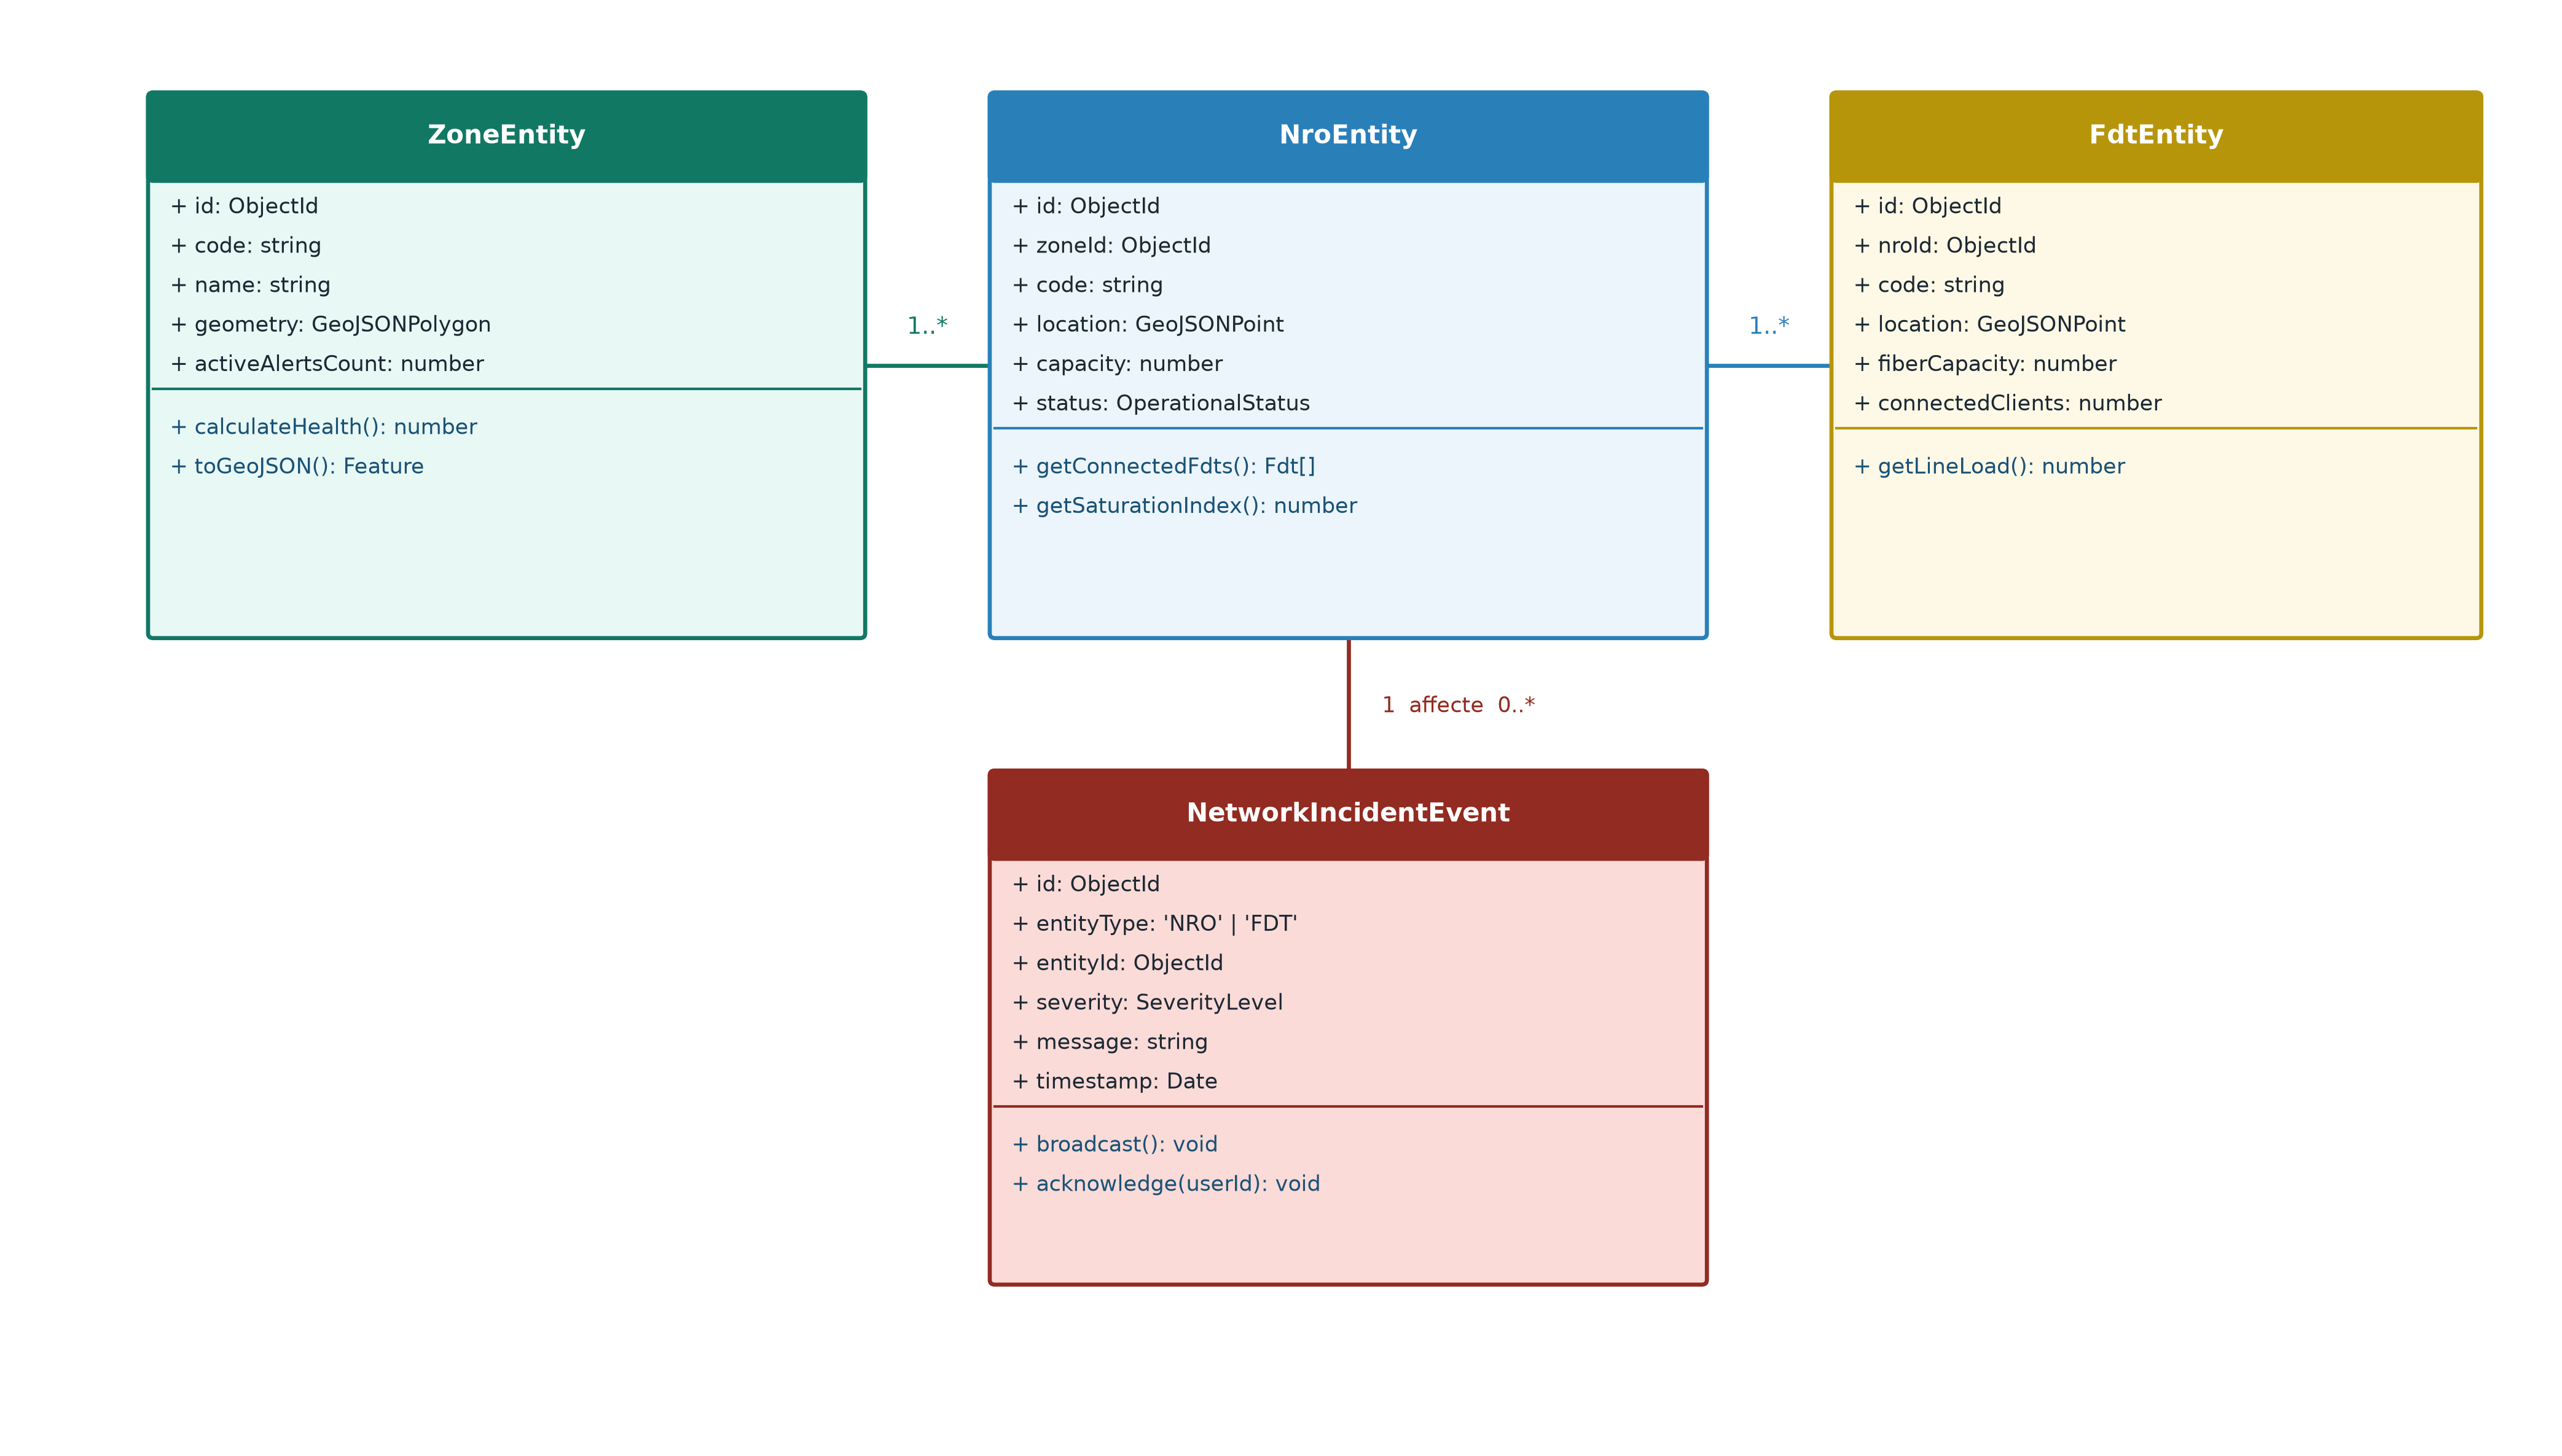
\includegraphics[width=15cm]{Images/ch4/map_layers_class.png}
 \caption{Diagramme de classes du domaine R\'eseau, Topologie et \'Ev\'enements}
 \label{fig:ch4-map-layers-class}
\end{figure}

\section{R\'ealisation technique et impl\'ementation}

\subsection{Gestion des donn\'ees g\'eospatiales sous MongoDB}
Pour optimiser les performances lors du rendu cartographique de milliers d'\'el\'ements optiques, nous avons exploit\'e les fonctionnalit\'es g\'eospatiales avanc\'ees de MongoDB :
\begin{itemize}
    \item \textbf{Format GeoJSON :} Les coordonn\'ees g\'eographiques sont stock\'ees sous forme d'objets conformes au standard GeoJSON (\texttt{Point} pour les NRO, FDT et contrats ; \texttt{Polygon} pour les p\'erim\`etres de zones).
    \item \textbf{Indexation \textit{2dsphere} :} Un index spatial 2dsphere a \'et\'e appliqu\'e sur le champ \texttt{location} de chaque collection, permettant des requ\^etes ultra-rapides bas\'ees sur des op\'erateurs sp\'ecialis\'es :
    \begin{itemize}
        \item \texttt{\$geoWithin} avec \texttt{\$box} pour r\'ecup\'erer uniquement les entit\'es visibles dans la fen\^etre d'affichage active de la carte ;
        \item \texttt{\$near} pour trouver les techniciens ou \'equipements les plus proches d'un incident.
    \end{itemize}
\end{itemize}

\subsection{Architecture de communication temps r\'eel (WebSockets)}
Le moteur temps r\'eel repose sur la passerelle \textbf{NestJS WebSocket Gateway (Socket.IO)} :
\begin{itemize}
    \item \textbf{Authentification du handshake WS :} Le jeton JWT est valid\'e d\`es l'\'etablissement de la connexion WebSocket.
    \item \textbf{Canaux segment\'es (\textit{Rooms}) :} Les clients rejoignent automatiquement des salles correspondant \`a leur zone (\texttt{zone\_<id>}). Ainsi, les \'ev\'enements d'une zone sp\'ecifique ne sont diffus\'es qu'aux utilisateurs habilit\'es, r\'eduisant drastiquement la consommation de bande passante.
    \item \textbf{R\'econciliation d'\'etat sur Flutter :} \`A la r\'eception d'un message Socket.IO, les providers \textbf{Riverpod} mettent \`a jour la liste des entit\'es en m\'emoire locale, d\'eclenchant une r\'e-animation cibl\'ee du marqueur concern\'e sur la carte.
\end{itemize}

\subsection{Interfaces utilisateur r\'ealis\'ees}

\subsubsection{Supervision cartographique multi-couches}
La figure~\ref{fig:ch4-ui-map} pr\'esente la carte interactive Flutter montrant les zones, les sous-r\'epartiteurs FDT et les marqueurs d'incidents.

\begin{figure}[H]
 \centering
 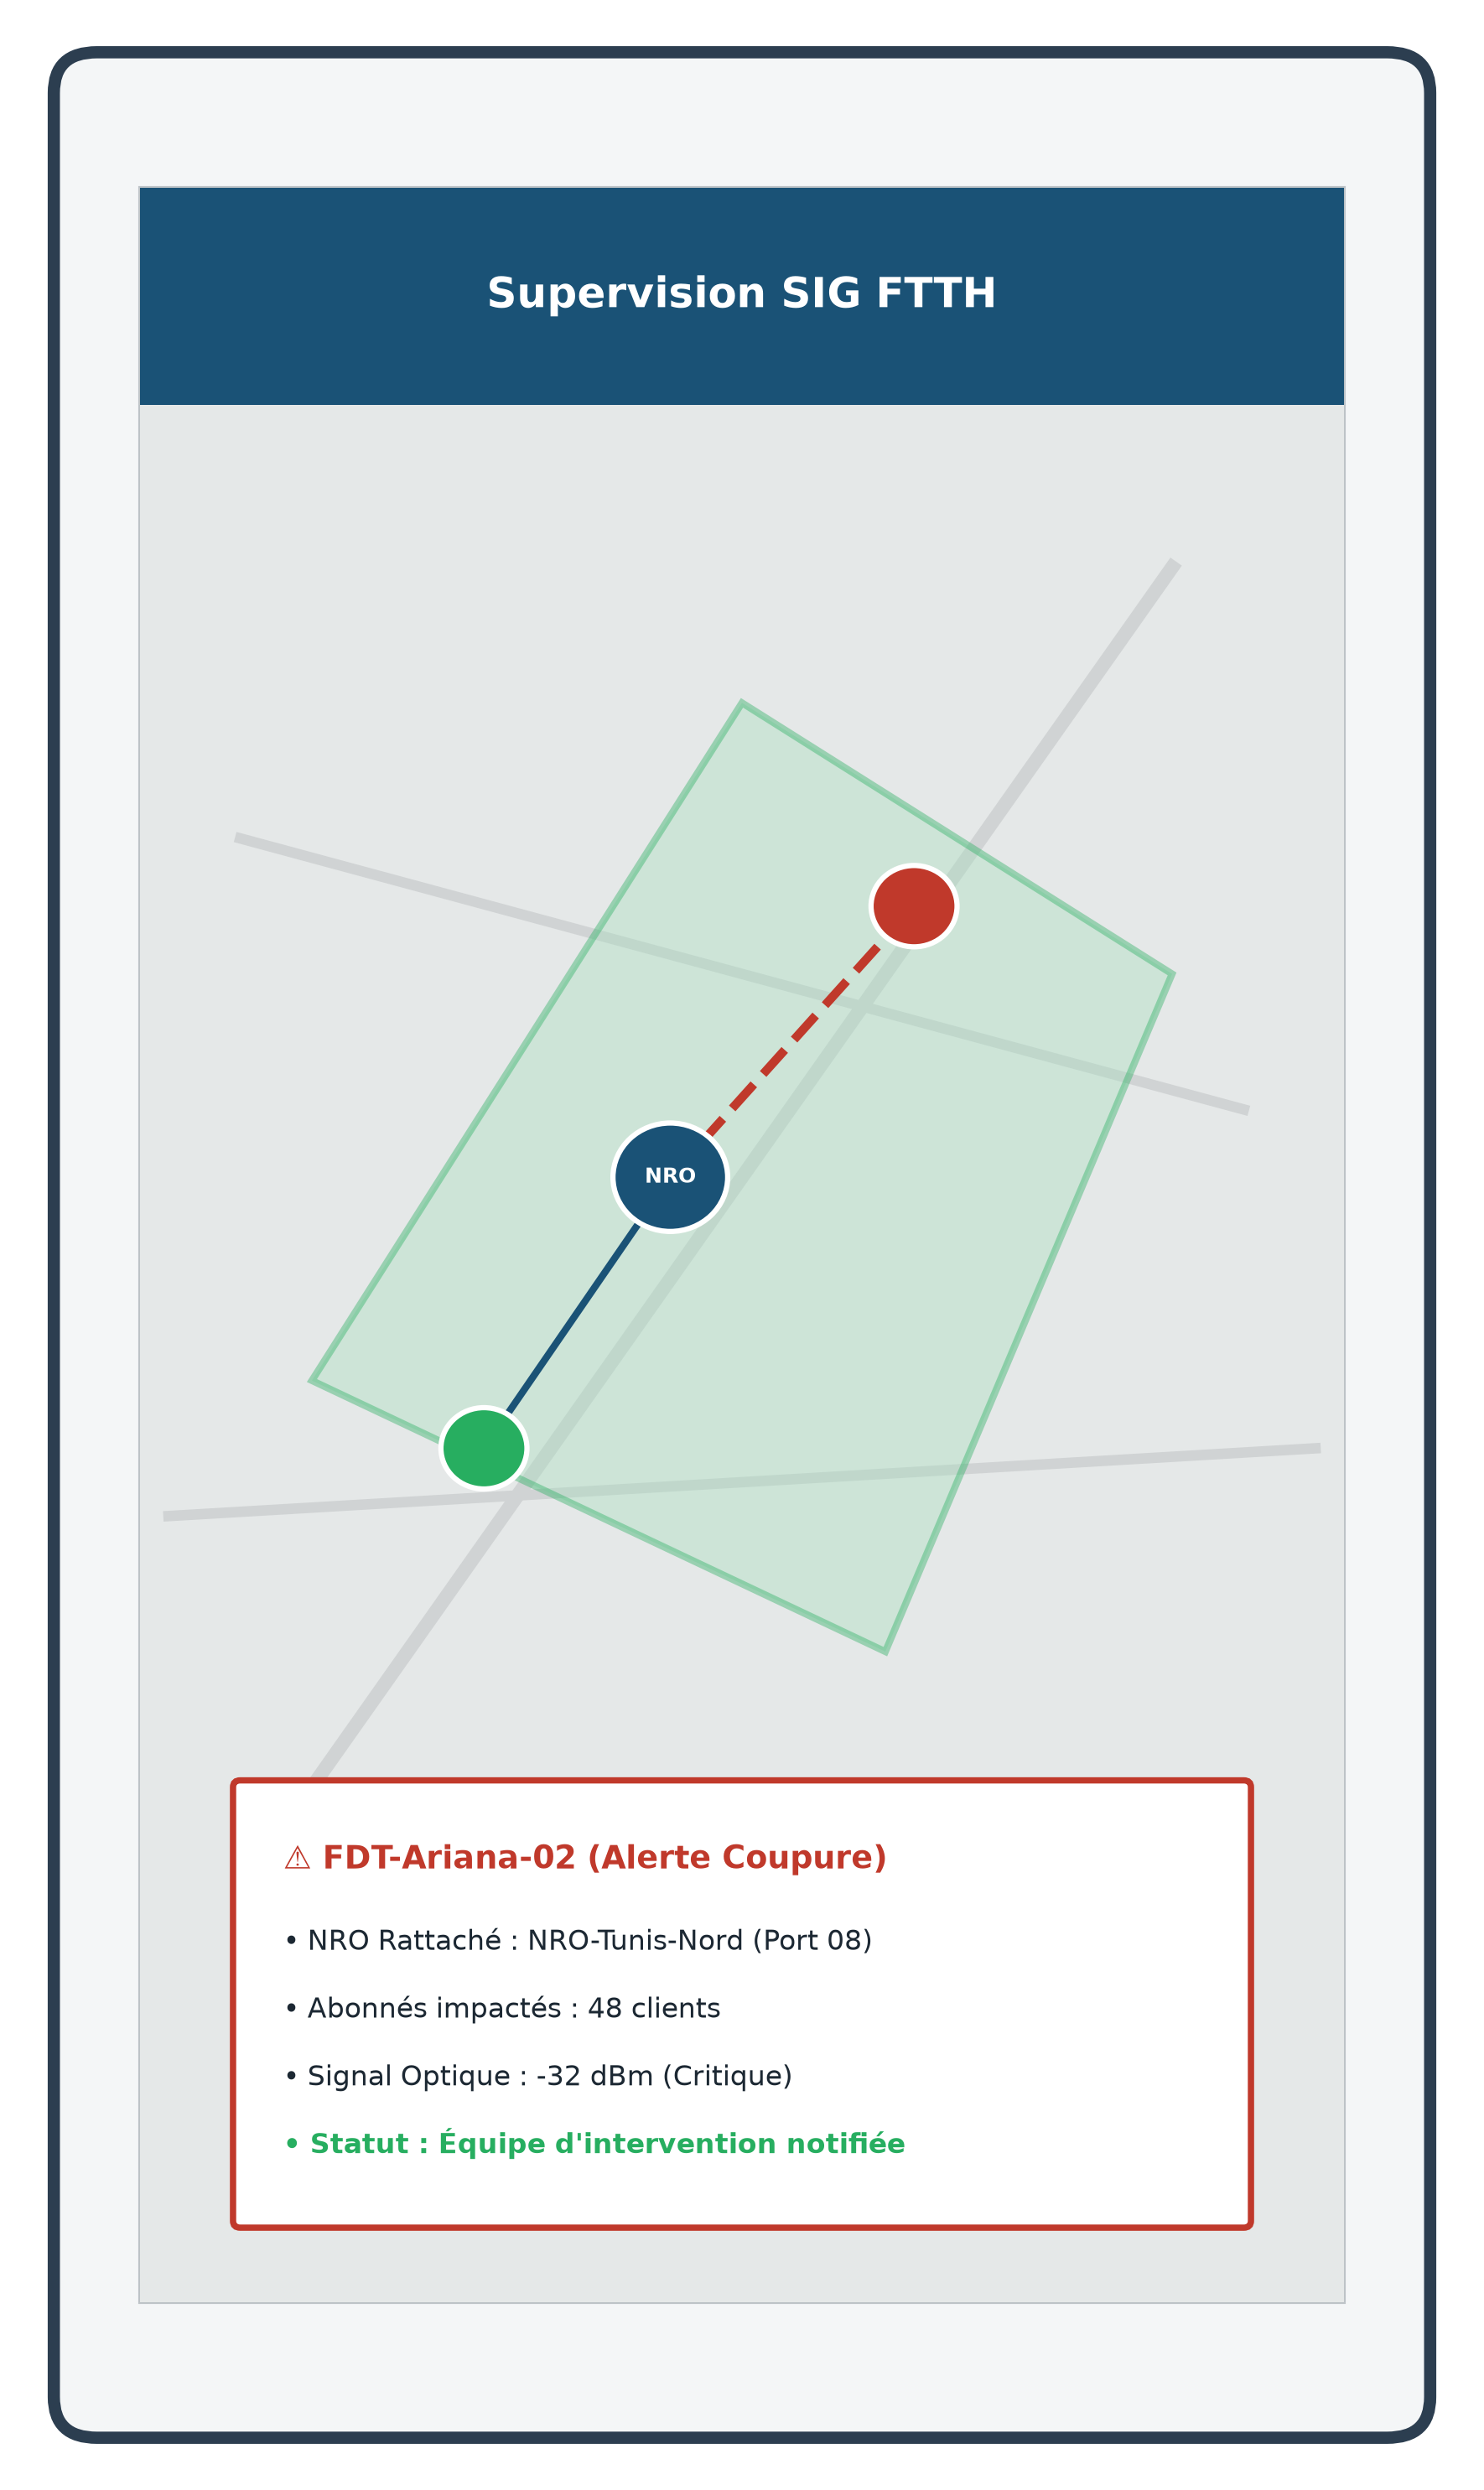
\includegraphics[width=12cm]{Images/ch4/ui_network_map.png}
 \caption{Interface de supervision cartographique interactive}
 \label{fig:ch4-ui-map}
\end{figure}

\subsubsection{Tableau de bord op\'erationnel (Dashboard KPI)}
La figure~\ref{fig:ch4-ui-dashboard} illustre le tableau de bord int\'egrant les r\'epartitions de pannes, les taux de disponibilit\'e par gouvernorat et l'historique des incidents.

\begin{figure}[H]
 \centering
 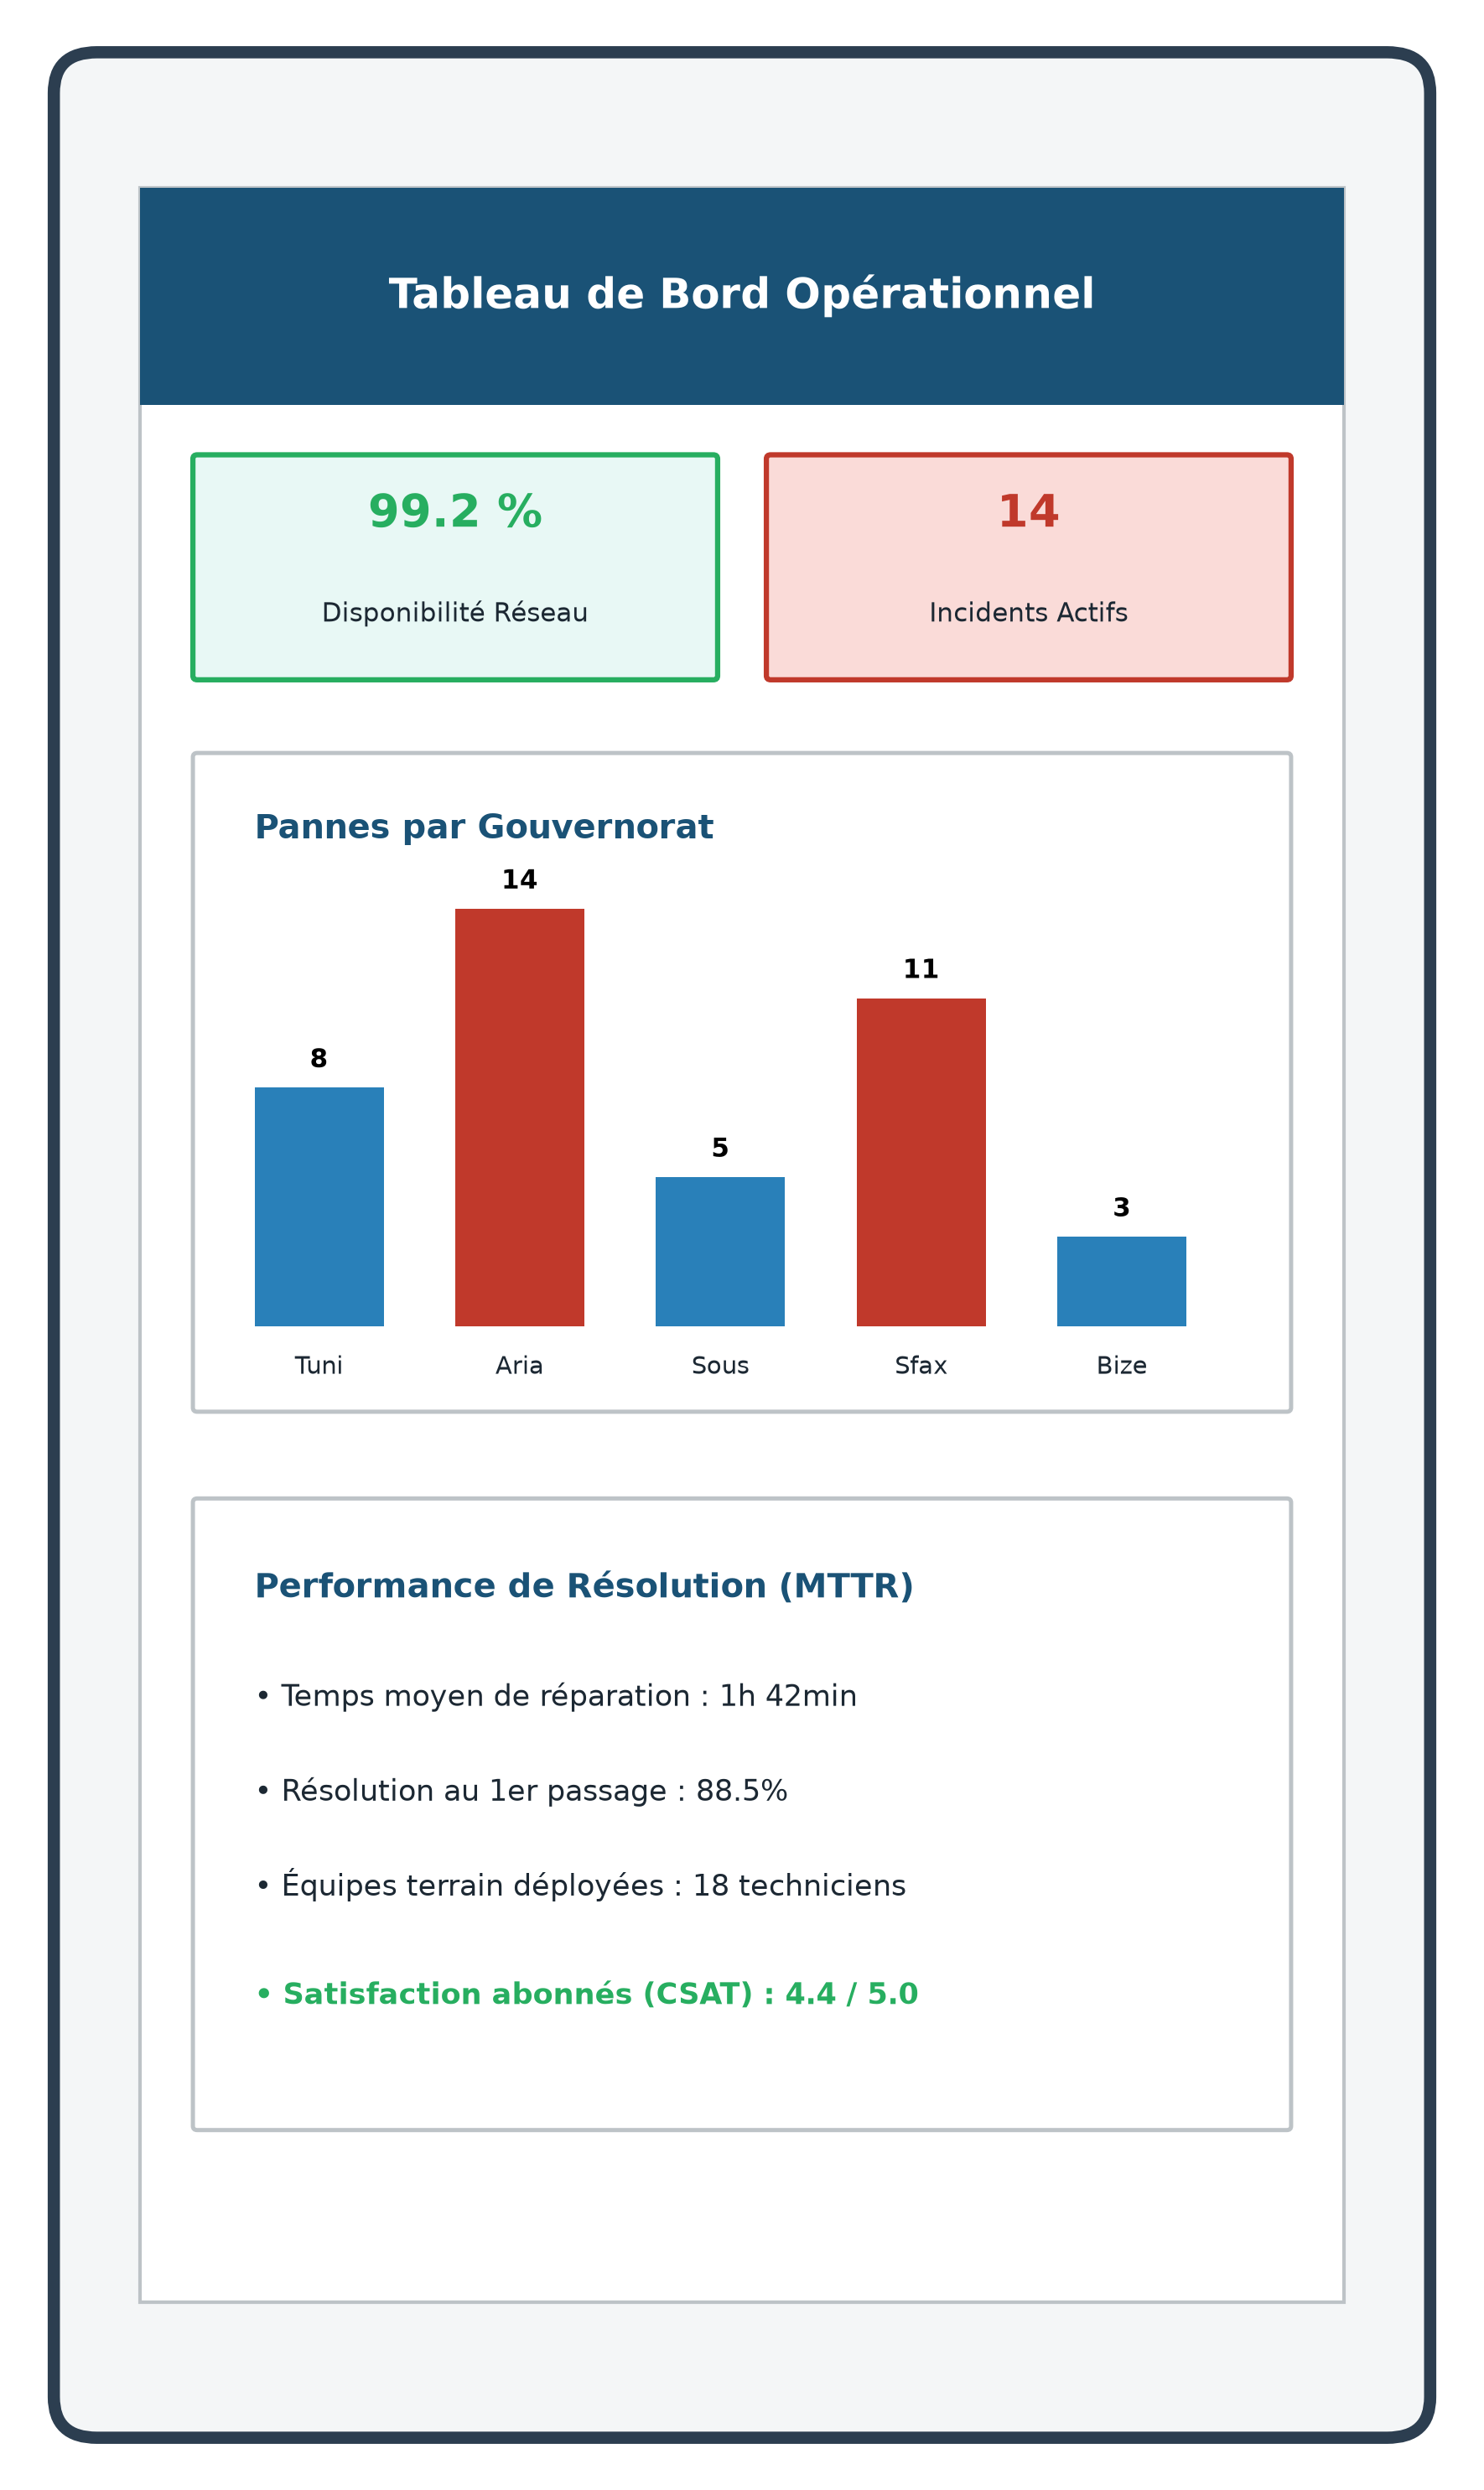
\includegraphics[width=12cm]{Images/ch4/ui_dashboard.png}
 \caption{Tableau de bord de pilotage op\'erationnel et m\'etriques KPI}
 \label{fig:ch4-ui-dashboard}
\end{figure}

\subsubsection{Centre de gestion des notifications et alertes}
La figure~\ref{fig:ch4-ui-notifications} montre l'interface de r\'eception et de filtrage des alertes temps r\'eel.

\begin{figure}[H]
 \centering
 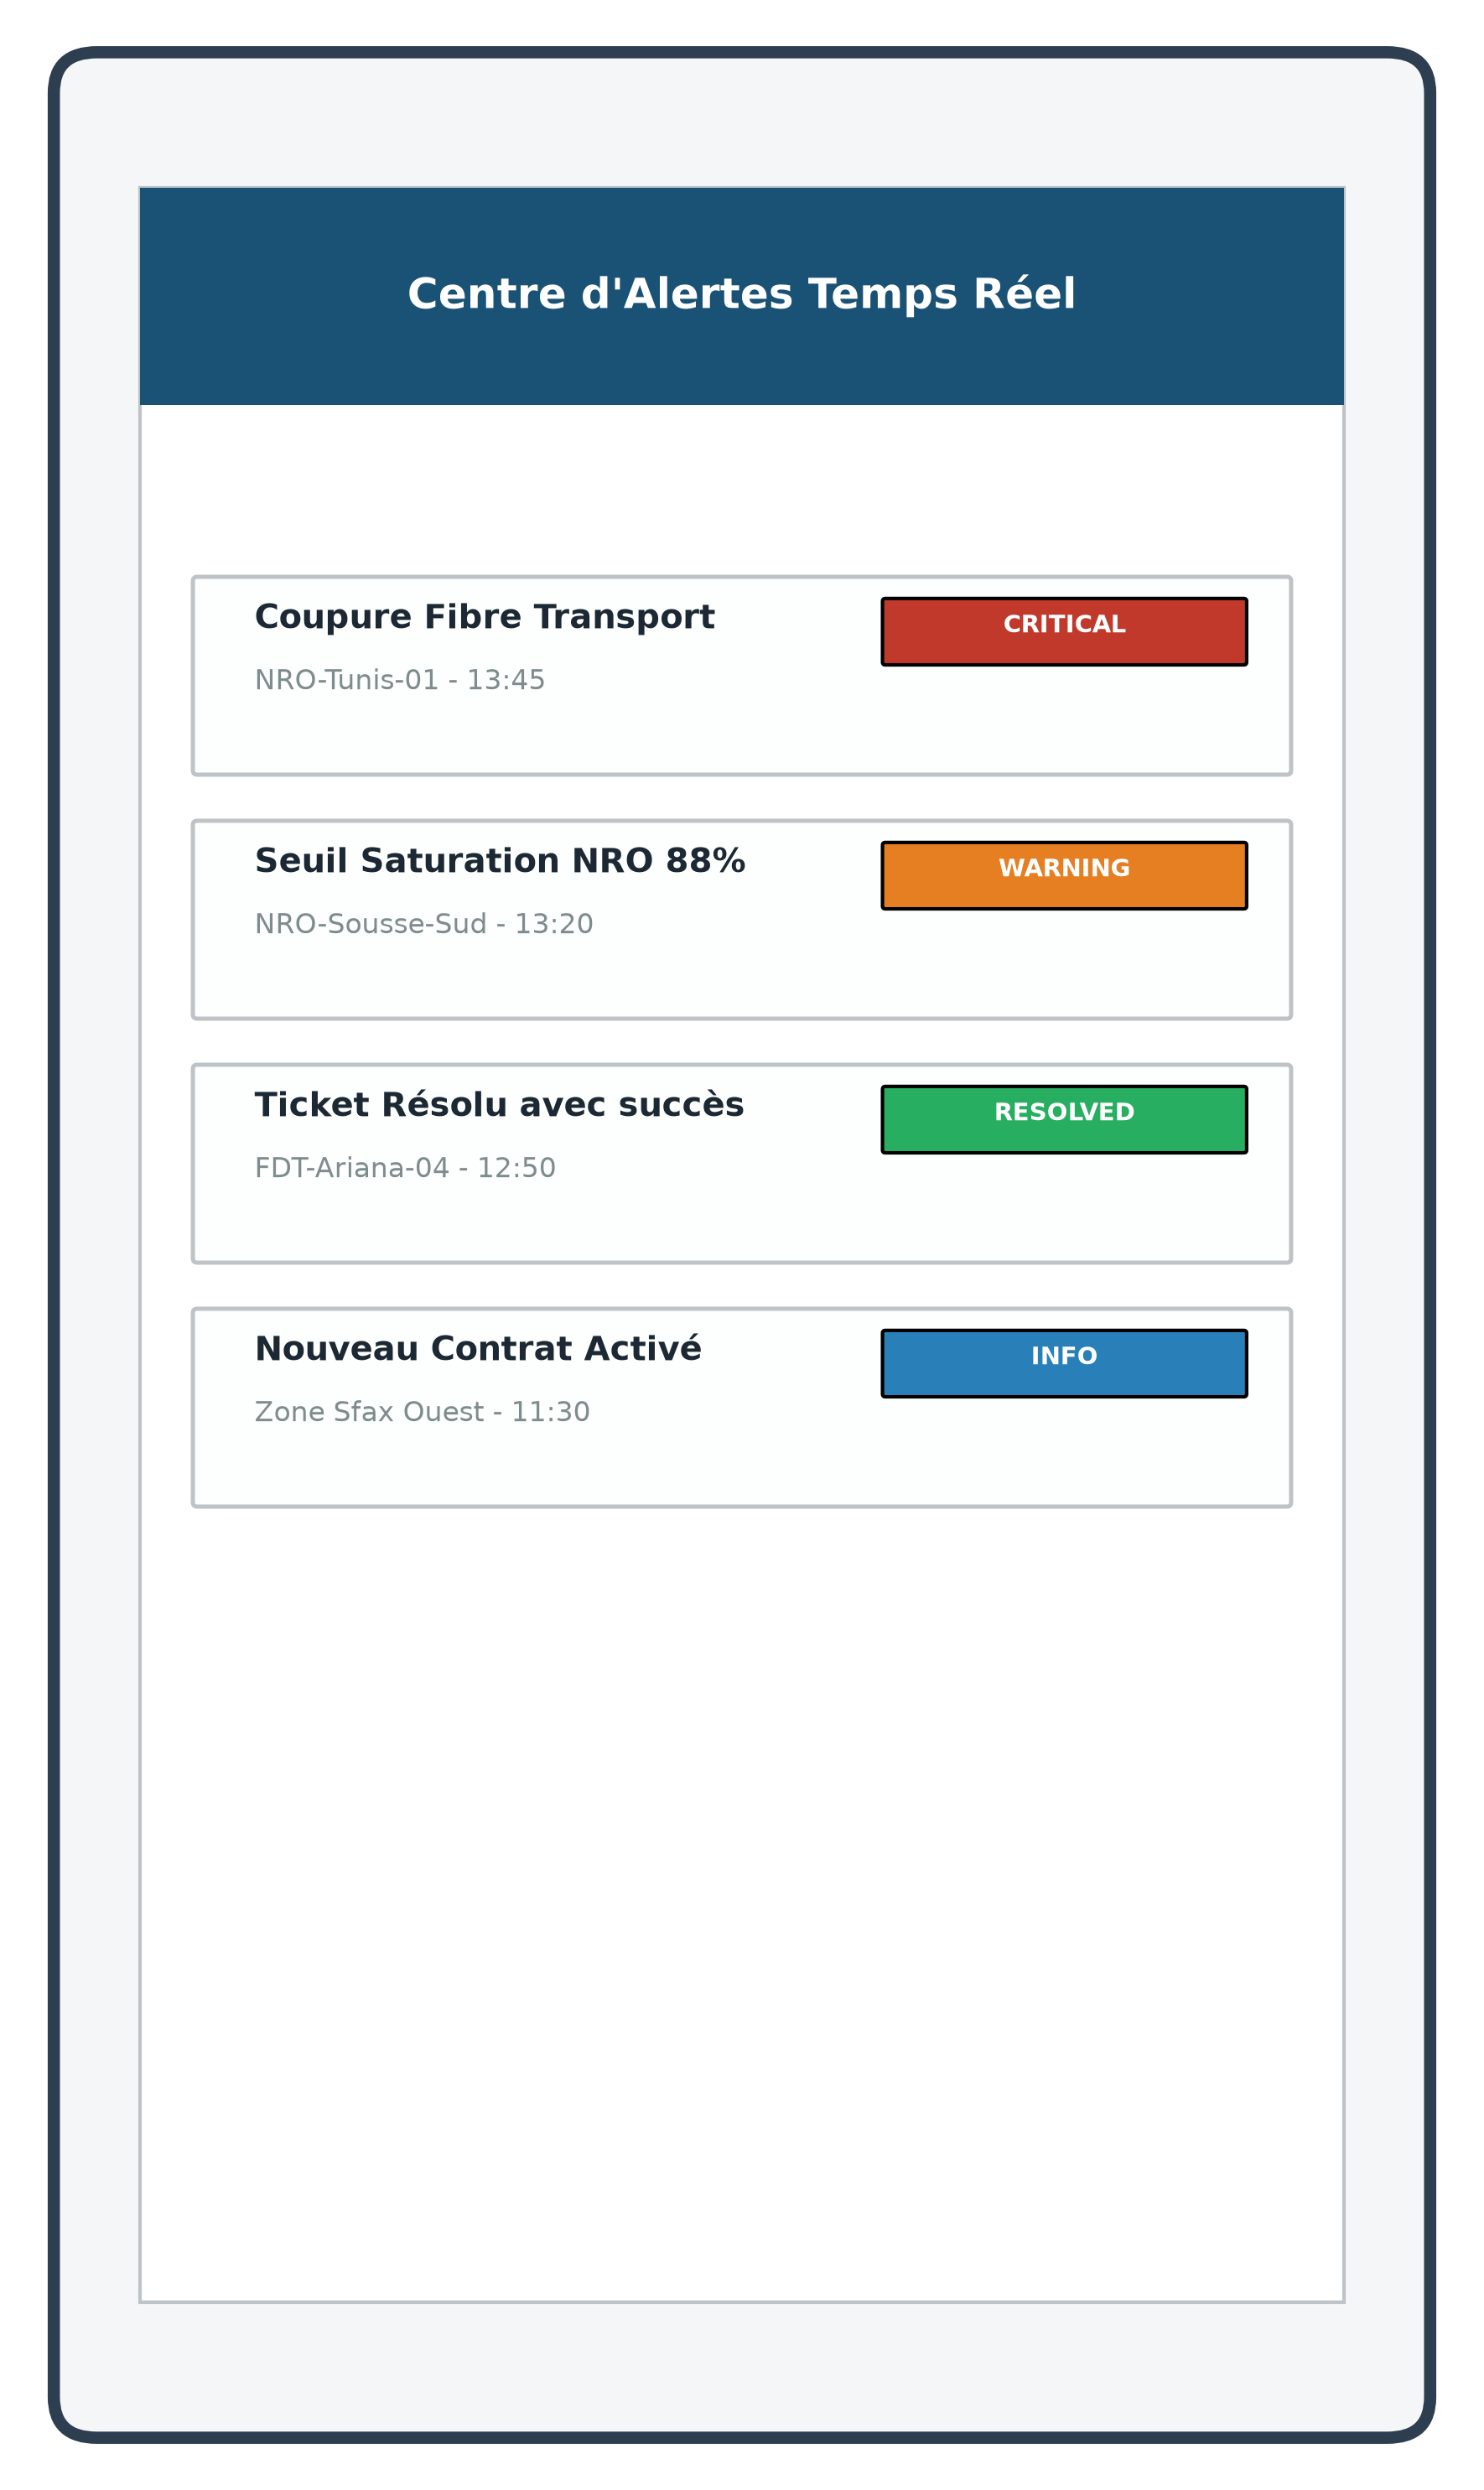
\includegraphics[width=10cm]{Images/ch4/ui_notifications.png}
 \caption{Interface du centre de notifications et alertes r\'eseau}
 \label{fig:ch4-ui-notifications}
\end{figure}

\section*{Conclusion}
La Release 2 a concr\'etis\'e la valeur m\'etier op\'erationnelle de la plateforme en offrant une exp\'erience cartographique r\'eactive, fluide et enrichie en temps r\'eel. L'int\'egration harmonieuse entre MongoDB g\'eospatial, la passerelle Socket.IO et les widgets \textit{flutter\_map} assure un suivi imm\'ediat de l'infrastructure optique. Le chapitre 5 pr\'esente l'\'etape finale du projet : l'adjonction de l'intelligence artificielle et l'industrialisation du syst\`eme.
